\documentclass[12pt,a4paper,oneside]{article}
\usepackage[colorlinks=true]{hyperref}
\usepackage[utf8]{inputenc}
\usepackage[czech]{babel}
\usepackage{graphicx}
\usepackage{pdfpages}
\textwidth 16cm \textheight 25cm
\topmargin -1.3cm 
\oddsidemargin 0cm
\pagestyle{empty}
\begin{document}
\title{Radiová meteorická detekční stanice RMDS02D}
\author{Jakub Kákona, kaklik@mlab.cz }
\maketitle

\begin{abstract}
Konstrukce softwarově definovaného přijímacího stanoviště pro záznam rádiových odrazů meteorů. Dokument obsahuje přehled technických parametrů stanice. Podrobná dokumenetace je u jednotlivých MLAB modulů použitých v konstrukci. Zařízení je určeno pro měřící síť Bolidozor. 
\end{abstract}

\begin{figure} [htbp]
\begin{center}
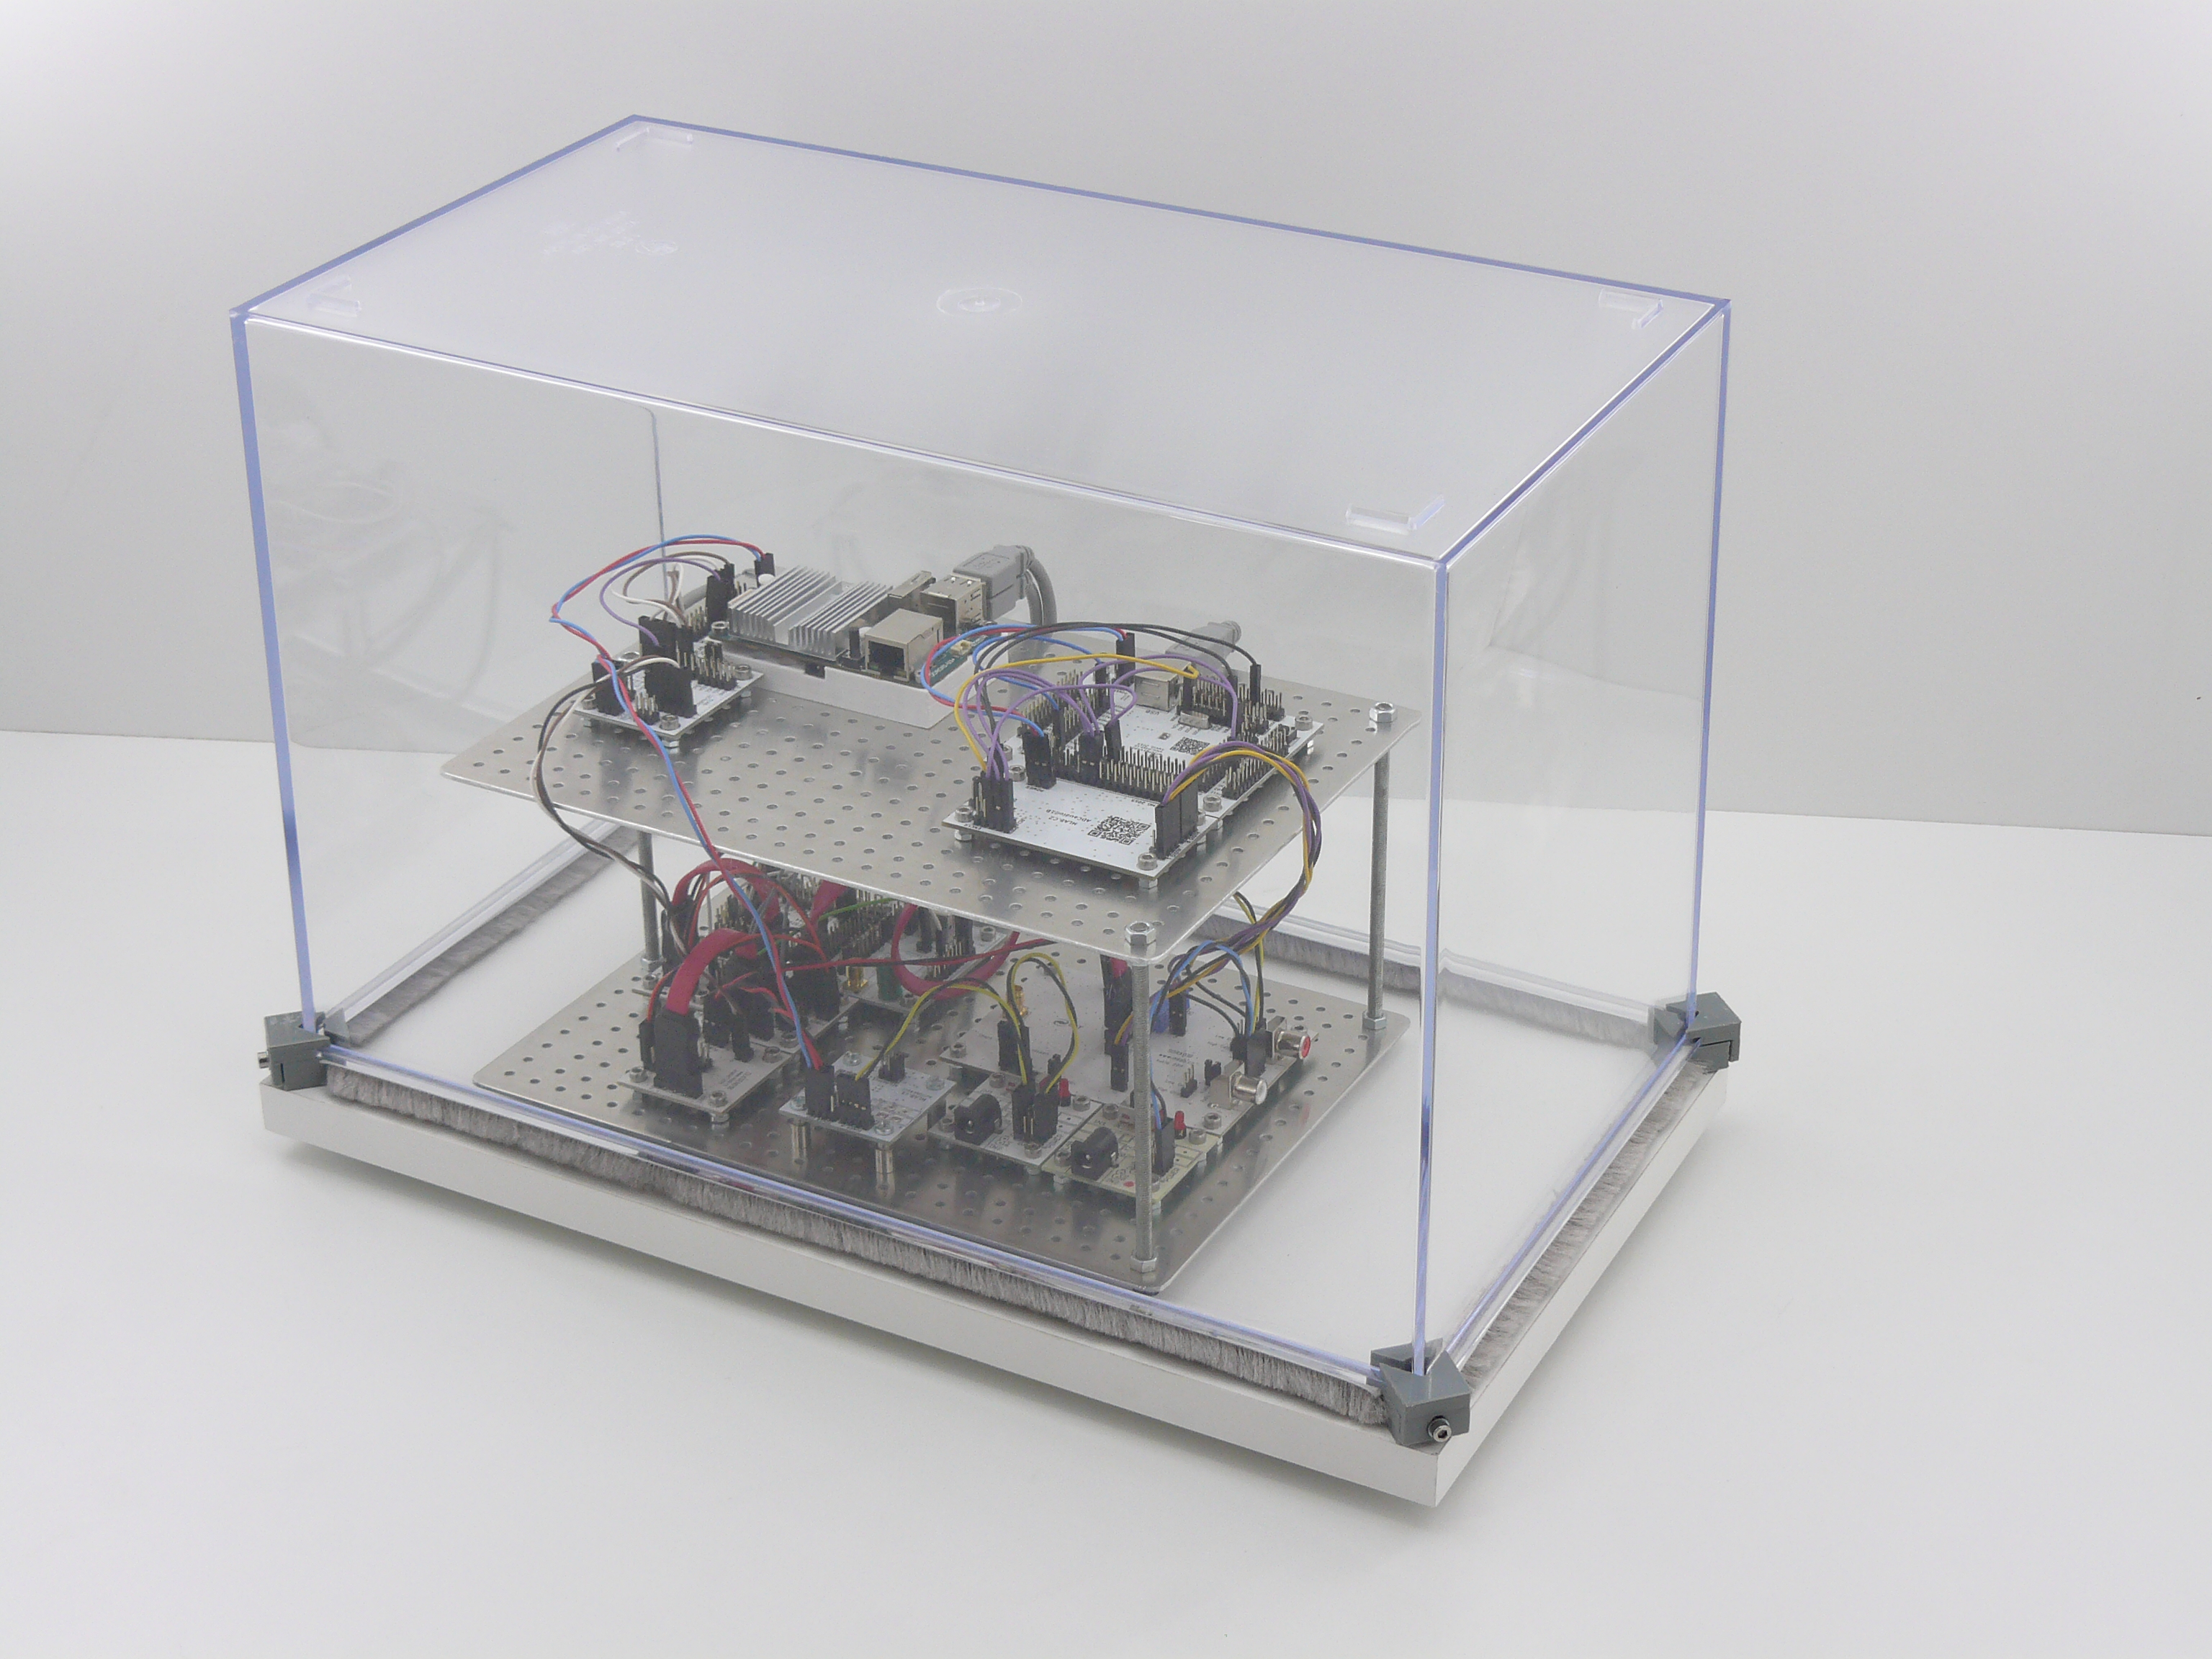
\includegraphics [width=120mm] {./img/RMDS02D_showcase1.JPG} 
\end{center}
\end{figure}

\begin{figure} [b]

\includegraphics [width=25mm] {./img/RMDS02C-QRcode.png} 
\end{figure}

\newpage
\tableofcontents

\section{Základní technické parametry}
\begin{table}[htbp]
\begin{center}
\begin{tabular}{|c|c|p{5cm}|}
\hline
\multicolumn{1}{|c|}{Parametr} & \multicolumn{1}{|c|}{Hodnota} & \multicolumn{1}{|c|}{Poznámka} \\ \hline
Napájení analogových obvodů & $\pm$12V &  cca 35mA \\ \hline
Napájení digitálních obvodů & 2x +5V &  2A \\ \hline
Napájení předzesilovače  & 9-12V &  500 mA \footnote{Chráněno vratnou PTC pojistkou 750mA na desce přijímače} \\ \hline
Pracovní Frekvenční rozsah  & 0,5 - 200 MHz & Obvykle 143.05 MHz $\pm$ 192 kHz \\ \hline
Vzorkování I/Q signálu  & 16bit@96kHz & \\ \hline
Celkový zisk & 60-90 dB & Volitelně podle konfigurace LNA \footnote{Lze ovlivnit jumperem na desce přijímače}\\ \hline
Celkové šumové číslo & $<$ 10 dB & \\ \hline
Minimální detekovatelný signál & -135dBm  &  Při konfiguraci v síti Bolidozor.\\ \hline
Přesnost časové synchronizace &  65ns (1$\sigma$) &  Používán signál GPS L1.\\ \hline
Rozlišení kontrolního měření frekvence LO &  0.1 Hz &  Přesnost je závislá na kvalitě signálu GPS.\\ \hline
\end{tabular}
\end{center}
\end{table}

\newpage

\section{Princip rádiové detekce meteorů}

Nejznámější metodou radiové detekce meteorů je metoda označovaná, jako dopředný rozptyl. Tento princip využívá rozptylu rádiových vln na ionizované stopě meteoru. Zdrojem rádiových vln je v takovém případě již existující vysílač (historicky to byly například televizní, nebo rozhlasové vysílače), který je umístěný pokud možno pod radiovým horizontem přijímače, tak aby nebyla slyšitelná jeho přímá vlna, která by mohla zahltit detekční stanici příliš intenzivním signálem. Pozorovatelné rádiové vlny se pak odrážejí prakticky výhradně od ionizovaných stop během jejich vzniku a i při následné rekombinaci iontů, to způsobuje vznik charakteristického signálu, který je pozorovatelný v blízkosti nosné frekvence vysílače. Většina těchto ionizovaných stop vzniká v horní atmosféře ve výškách okolo 100 $\pm$ 20 km.  

\begin{figure} [htbp]
\centering
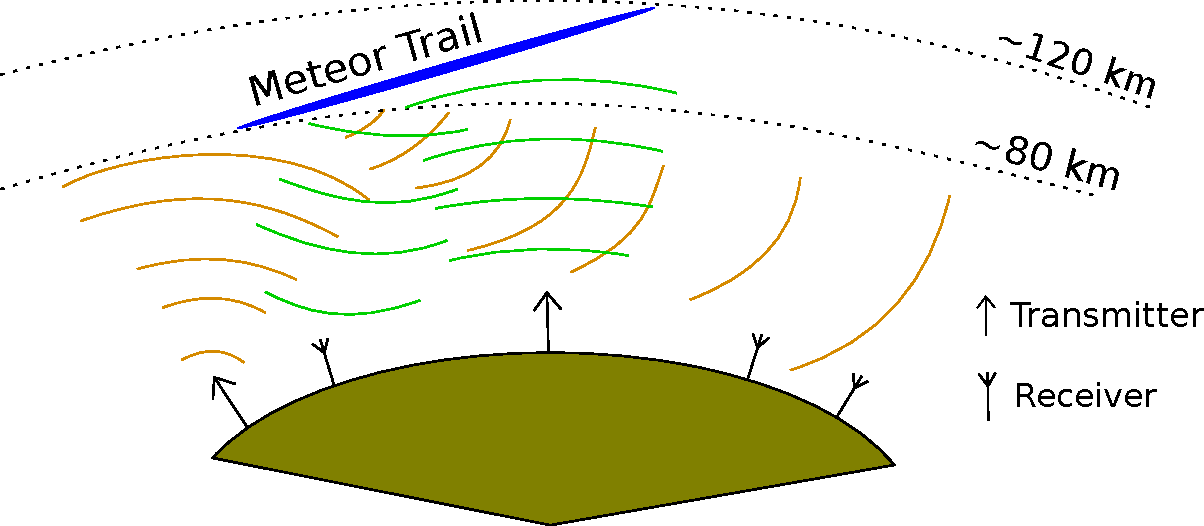
\includegraphics [width=120mm] {./img/Meteor_detection.pdf} 
\caption{Znázornění šíření signálu, při použití multistatického systému.}
\end{figure}

Přímý odraz od samotného meteoroidu není obvykle detekovatelný z několika důvodů, jednak materiál meteoroidu není obvykle dostatečně reflexivní pro radiové vlny a zároveň jeho rozměr je velmi malý (0.05 - 200mm) a je tedy zlomkem vlnové délky rádiových vln. Tato malá zrníčka prachu ale vstupují do horních vrstev atmosféry supersonickými rychlostmi. Což způsobuje vznik rázové vlny, prudké ohřátí plynu a jeho ionizaci. Tato rázová vlna navíc dosahuje do velké vzdálenosti od samotného zrníčka minimálně jednotky metrů, což je již rozměr dostačující k interakci s radiovou vlnou. Ovšem vzhledem k supersonickým rychlostem pohybu meteoroidu má odražená vlna velký dopplerovský posuv a intenzita odrazu je navíc na začátku slabá, proto je v této fázi těžké odraz správně detekovat. Nicméně v zápětí se doplerovský posuv vlivem snížení rychlosti zmenšuje až k frekvenci vysílače, nebo i mírně pod ní. Pak je možné pozororovat relativně silný odraz. Tento jev se pak nazývá "head echo efekt" a je způsoben odrazem signálu od čela plazmatického tubusu vznikajícího v atmosféře v těsné blízkosti meteoroidu. Je zřejmé, že tento jev nebude pozorovatelný  vždy, neboť závisí na geometrii průletu meteoru vzhledem k vysílači a k detekční stanici. A v některých případech proto bude pozorován pouze odraz od stopy bez výrazných dopplerovských jevů. 

Při popisu principu této metody detekce se často můžeme setkat s pojmem meteorický radar.  Ovšem slovo RADAR je ve skutečnosti zkratka pro 'radio detection and ranging', ovšem vzdálenost a směr mohou být získána pouze z dat získaných ze skupiny přijímačů. Jedna přijímací stanice proto není případem radarového systému.  Samostatný přijímač je proto schopen pouze změřit četnosti meteoroidů vstupujících do atmosféry v prostoru osvětleném vysílačem. Některé další charakteristiky je sice možné získat zpětnou analýzou záznamů odrazů, ale zdánlivě jasné údaje, jako vazba mezi intenzitou odrazu a hmotností meteoroidu je komplikovaná problémy s neznámou polarizací signálu, trajektorií meteoru a pokrytím oblohy signálem z vysílače.
    
Jednou z hlavních výhod rádiové detekce meteorů je fakt, že tato metoda funguje nezávisle na počasí i jasu oblohy. Funguje proto jak ve dne, tak i v noci. Zvolením vhodné frekvence a výkonu vysílače je navíc možné detekovat i meteory, které by jinak byly příliš slabé k pozorování okem, nebo celooblohovou kamerou. Počty rádiově detekovaných meteorů jsou proto obvykle řádově vyšší, než u optického pozorování. 

\subsection{Vysílač GRAVES}

Využití signálu z francouzského vojenského radaru GRAVES má od klasického způsobu pozorování s využitím televizních vysílačů výhodu především ve stálosti vysílání vojenského systému a v obrovském výkonu, kterým radar vysílá a jeho signál tak lze použít téměř po celé Evropě. 
Bistatický radar GRAVES je umístěn ve Francii na lokátoru JN27SI. Vysílá na frekvenci 143.050 MHz CW 24 hodin denně (vyzářený výkon je několik MW). Jeho cílem je tzv. space surveillance, což znamená mapování umělých objektů na oběžné dráze Země. 

\begin{figure} [htbp]
\centering
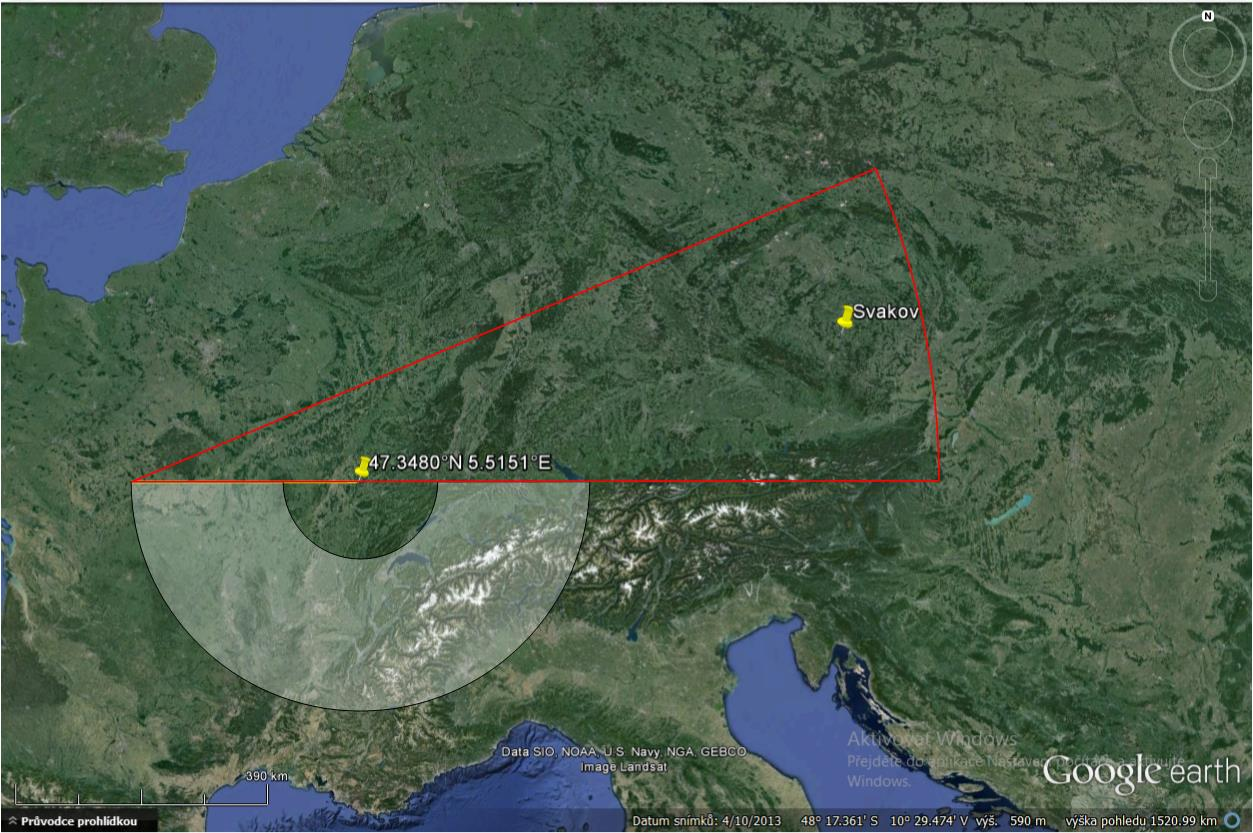
\includegraphics [width=120mm] {./img/graves_range.jpg} 
\caption{Mapa zobrazuje šedivou oblast, která je projekcí vyzařovacího diagramu radaru na sférickou plochu 100km nad Zemí. Červený rádius pak vymezuje oblast, ve které je šedivá plocha nad horizontem.}
\end{figure}

Vysílač radaru má čtyři separátní fázované anténní soustavy. Každá anténní soustava pokrývá 45 stupňů v azimutu. Radar pokrývá pouze jižní oblohu, 90 až 270 stupňů. Horizontální svazek je široký 7.5 stupně. Každý sektor je tedy rozdělen 6 dílů. Do každého dílu sektoru vysílá radar 1,6 sekundy. Oskenovat celý sektor tedy trvá 19,2 sekundy a každý sektor je skenován 4500 krát za 24 hodin. Všechny 4 sektory vysílají najednou. Podle dostupných údajů \cite{GRAVES_book} by měl být vyzařovací úhel ve vertikální rovině 25 stupňů. Dle sledování PE1ITR jsou odrazy od mesíce dobře slyšitelné od 15 do 40 stupňů. Sekvence vysílání do sektorů je vázána na UTC, proto lze zjistit, kam právě radar vysílá.


\section{Konstrukce detekční stanice}

Za účelem systematického sledování meteorů v síti Bolidozor a měření kvalitních dat je vyvíjena specializovaná detekční stanice. Aktuálně je v provozu několik verzí. Následující verze vznikají obvykle přidáním dalších modulů, pozorovatel si tak může pro začátek pořídit základní verzi a s ní trvale pozorovat nebo ji později přidáním dalších modulů doplnit až na nejnovější verzi. 


\begin{figure}[htbp]
\begin{center}
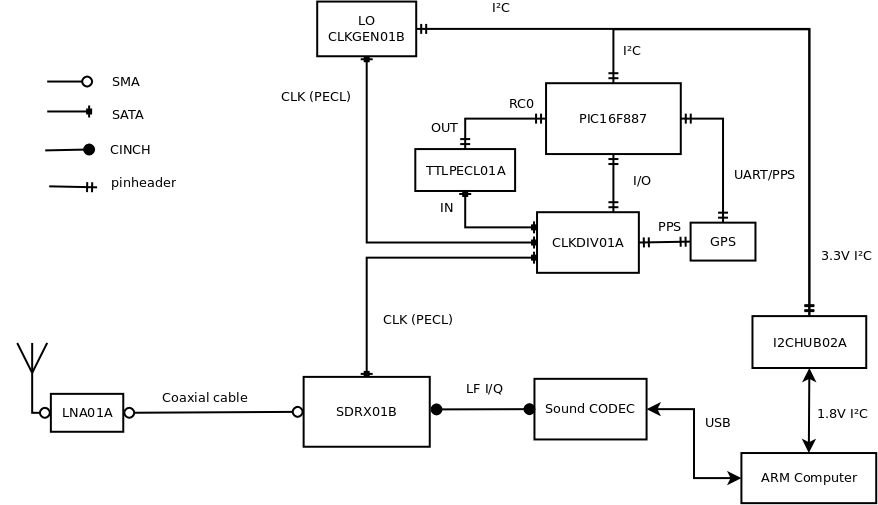
\includegraphics [width=130mm] {../../SCH/RMDS02C_system.png} 
\end{center}
\caption{Blokové schéma zapojení jednotlivých modulů detekční stanice.}
\end{figure}


\subsection{Přijímací anténa}

Detekční stanice většinou využívá modifikovanou GroundPlane anténu s jedním radiálem natočeným směrem k vysílači radaru GRAVES. Jde základní anténu, kterou lze intastovat na většině stanic. Její hlavní předností jsou malé rozměry, takže umožňuje i instalaci na balkon, terasu a podobně. Díky svojí primitivní konstrukci je  vhodná i pro začátečníky.

Nevýhodou je že namá celkově příliš dobrý zisk a její vyzařovací charakteristika má v zenitu ostrou nulu, to znamená že bude velmi špatně detekovat meteory, prolétající nad hlavou na rozdíl od klasického vizuálního pozorování. 

\begin{figure}[htbp]
\begin{center}
\includegraphics [width=120mm] {./img/GP143MHz_plastic.png} 
\end{center}
\caption{Konstrukce antény používané na detekční stanici.}
\end{figure}

Přijímaný signál je za anténou zesílen laděným nízkošumovým zesilovačem. Tato konstrukce využívá předzesilovač LNA01A\cite{LNA01A_wiki}.

LNA01A je předzesilovač konstrukčně určený pro detekci meteorů v pásmu 2m. Jeho přínos spočívá v zesílení signálu z antény a tím ke snížení vlivu vlastního šumu přijímače. Navíc také zmenší komplikace spojené s přenosem signálu koaxiálním kabelem (Vyváží útlum kabelu a je proto možné použít i levnější koaxiální kabel typu RG58) 

\subsection{SDR přijímač}

V přijímací stanici je využíván přijímač MLAB SDRX01B \cite{SDRX01B_pdf}. Jde o SDR přijímač zkonstruovaný původně pro účely amatérské radioastronomie a je proto optimalizovaný pro realizaci škálovatelných rádiových systémů. Přijímač vyžaduje externí lokální oscilátor, který je v případě této konstrukce realizovaný zapojením modulu CLKGEN01B s obvodem Si570, který je řízen přes sběrnici I2C.  Frekvence tohoto lokálního oscilátoru je měřena 3x za minutu a logována do souboru. Po změření se navíc frekvence automaticky koriguje na nastavenou hodnotu. Fázový šum lokálního oscilátoru je maximálně –105~dBc/Hz (Při offsetu 100~Hz)

\begin{figure}[htbp]
\begin{center}
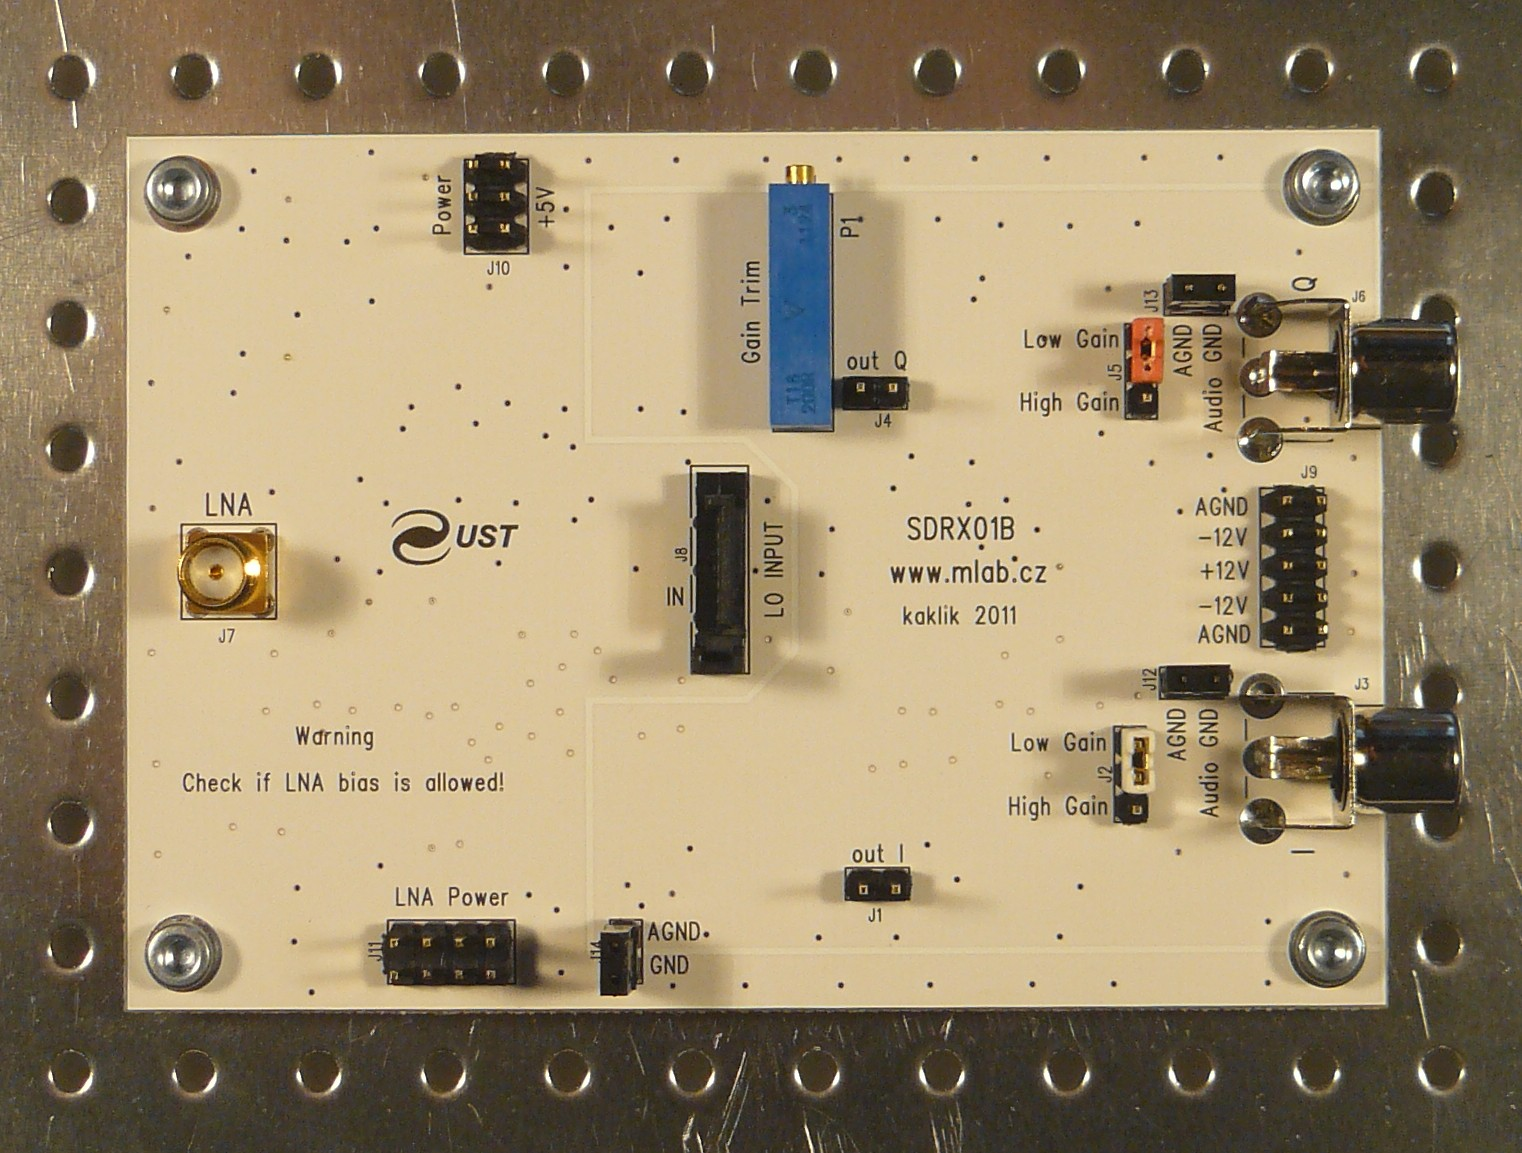
\includegraphics [width=120mm] {./img/SDRX01B_Top_Big.JPG} 
\end{center}
\caption{Hlavní modul přijímače SDRX01B}
\end{figure}

Díky měření frekvence lokálního oscilátoru je ve stanici v podstatě obsažena GPSDO kmitočtová reference, která napájí přijímač. Výstupem přijímače je tak komplexní I/Q signál, který je v této verzi stanice digitalizován externí USB zvukovou kartou Behringer UCA 202 U-CONTROL. Tento audio kodek vzorkuje 48kHz s rozlišením 16bit ve dvou kanálech.  Zvuková karta bude v následující verzi stanice nahrazena digitalizační jednotkou SDR-Widget. Která už může mít vzorkovací hodinový signál též odvozen od hlavního lokálního oscilátoru. 

\subsection{Časová synchronizace}

Časová synchronizace je velmi dúležitá ve vědeckých měřeních. Konstrukce využívá dvě metody časové synchronizace NTP a signál z GPS.  NTP je využíváno pro časovou synchronizaci systémových hodin staničního počítače a používá se i pro generování názvů výstupních datových souborů. Přesnost tohoto synchronizačního kanálu závisí na kvalitě internetového připojení, resp době pingu k NTP serveru.  Proto je na stanici zaveden ještě zdroj časových značek z GPS, který umožňuje značkovat výstupní data s rozlišením až na vzorkovací frekvenci digitalizační jednotky. 
Jako GPS přijímač je ve stanici využíván MLAB modul GPS01A s čipsetem uBlox-LEA6. Použitá GPS anténa je keramická patch s integrovaným předzesilovačem.

\subsubsection{Měření frekvence lokálního oscilátoru}

Stanice je vybavena automatizovaným systémem kontroly lokálního oscilátoru. Zařízení umožňuje měření frekvence lokálního oscilátoru oproti dlouhodobému časovému normálu z GPS. Měření se provádí tak, že signál z lokálního oscilátoru generovaného modulem CLKGEN01B se vydělí modulem CLKDIV01A a vydělený výstupní signál je veden do čítače v PIC16F887. Kde jsou na hrubo počítány tako vydělené hodinové pulzy. 
Modul GPS01A je pak nastaven tak, aby generoval 100us dlouhý impuls každých celých 10s UT.  Tento impuls je pak využit ke zahradlování děličky CLKDIV01A.  Zároveň impuls vede na vstup přerušení PIC16F887 a ten pak provede vyčtení čítače a interních stavů děličky tím, že projde všechny možné dělící poměry a přečte výstupní stav děličky. Výsledkem je absolutně změřený počet pulzů za 10s.  Toto číslo je následně uloženo v registrech mikrokontroleru PIC16F887. Vyčtení těchto registrů proběhne ze staničního počítače přes sběrnici I2C každou 5. 25. a 45. sekundu UT času. \footnote{Měření je takto rozloženo díky tomu, že obsluha I2C probíhá také pod přerušením a při vyčítání může dojít k poškození měřené hodnoty vynecháním přerušení obsluhy čítače.}
Protože při zahradlování děličky dojde k odpojení lokálního oscilátoru od směšovače v SDRX01B, tak na výstupním signálu se objeví impuls s širokým frekvenčním spektrem, který slouží jako časová značka ve výstupních datech.  Časová synchronizace tak zároveň přesně značkuje výstupní data hodinami odvozenými z GPS signálu. Tvar těchto časových značek je navíc odvozen od impulzní odezvy přijímacího řetězce, takže na něm lze pozorovat případné nežádoucí změny parametrů. 

\subsection{Staniční počítač}

Jako staniční počítač je využíván Hardkernel ODROID-U3, což je čtyřjádrový počítač postavený na architektuře ARM. K tomuto počítači je ještě obvykle připojen USB flash disk, který slouží jako krátkodobé uložiště pro zaznamenaná data.  Technické parametry použitého ARM počítače jsou následující: 

\begin{itemize}
\item 1.7GHz Quad-Core processor and 2GByte RAM
\item 10/100Mbps Ethernet with RJ-45 LAN Jack
\item 3 x High speed USB2.0 Host ports
\item Audio codec with headphone jack on board
\item GPIO/UART/I2C ports
\end{itemize}

Komponenty stanice jsou k počítači připojeny přes rozhraní USB: (Zvuková karta, GPS přijímač) a přes rozhraní I2C: (Lokální oscilátor, měření frekvence)

\begin{figure}[htbp]
\begin{center}
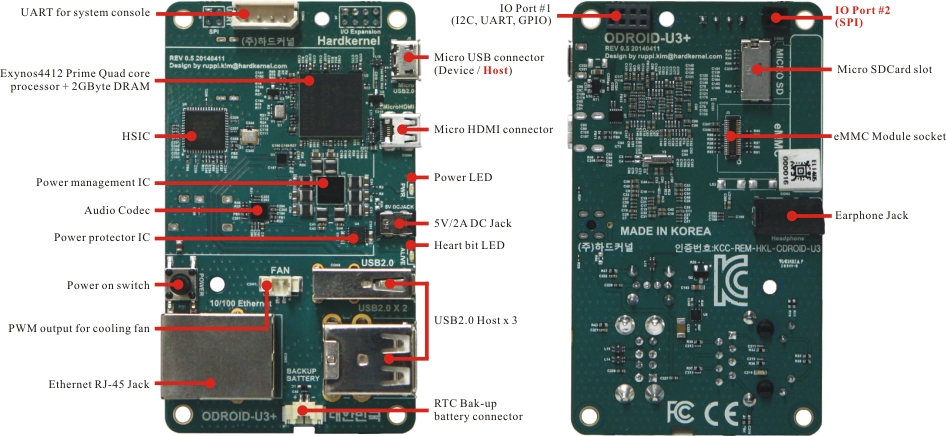
\includegraphics [width=140mm] {./img/u3rev05boarddetail.jpg} 
\end{center}
\caption{Deska počítače Hardkernel ODROID-U3}
\end{figure}

\section{Software stanice}

Na staničním počítači je nainstalovaný operační systém linux Lubuntu 14.04 LTS včetně grafického rozhraní xfce.  Grafické rozhraní je na stanici využíváno pro zobrazování stavových informací. (živý waterfall, stav GPS, stav uploadu dat). S datovým tokem z přijímače je zacházeno jako s širokopásmým audio signálem. Proto je pro rozvod  datového toku použit audiosystém JACK. Příklad rozvodu signálu je na obrázku \ref{qjackctl}.

\begin{figure}[htbp]
\centering
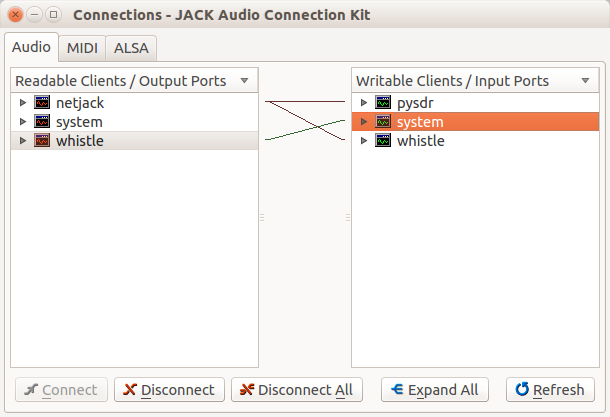
\includegraphics [width=120mm] {./img/JACK_audio.png} 
\caption{Rozvod audio signálu v systému JACK.}
\label{qjackctl}
\end{figure}

Jack audio server navíc umožňuje přenášet stream přes lokální síť ethernet a aktuální tok spektra z přijímače je tak možné sledovat i na jiných počítačích viz obr. \ref{Pysdr}.

\begin{figure}[htbp]
\centering
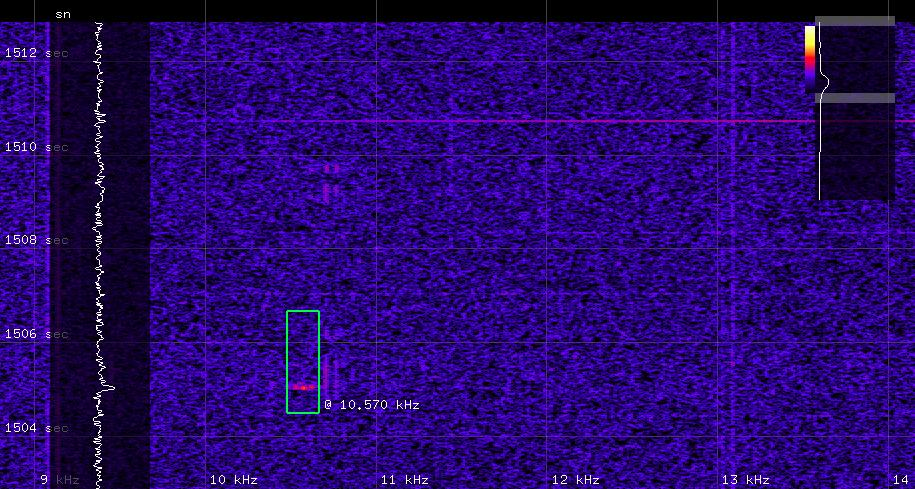
\includegraphics [width=120mm] {./img/meteor_pysdr.jpg} 
\caption{Vzdálené zobrazení toku spektra v programu PySDR. S meteorem označeným MIDI packetem.}
\label{Pysdr}
\end{figure}

\subsection{Záznam dat}

Data jsou na stanici zaznamenávána programem radio-observer, který běží jako klient systému jack, počítá FFT spektra a detekuje meteory podle intenzity signálu v oblasti, kde je předpokládán signál od vysílače. Pokud v této oblasti dojde ke zvýšení intenzity signálu o prahovou hodnotu nad šumem tak je detekován meteor.  Při detekci meteoru vznikne několik záznamů, jednak náhled na frekvenční oblast spektra, kde meteor byl detekován. Potom záznam surových vzorků z přijímače a také záznam do metadatového souboru s parametry signálu detekovaného meteoru (délka odrazu, intenzita signálu, atd.). Datové výstupy jsou ve formátu FITS s kompresí RICE, buď jako navzorkované signály a nebo předpočítané spektrogramy. Všechna naměřená data jsou veřejně dostupná na datovém serveru. 

\subsection{Odesílání záznamů}

Naměřená data jsou ještě na stanici setříděna do stromové adresářové struktury podle času. A následně uploadována přes rsync na hlavní datový server space.astro.cz.

\subsection{Správa stanice}

Na stanici běží ještě další pomocné aplikace, jako sshd server, pro vzdálený přístup a skripty pro ladění a kontrolu lokálního oscilátoru.


\begin{thebibliography}{99}
\bibitem{GRAVES_book}{GRAVEs source book} 
\href{http://www.fas.org/spp/military/program/track/graves.pdf}{http://www.fas.org/spp/military/program/track/graves.pdf}

\bibitem{LNA01A_wiki}{Nízkošumový zesilovač LNA01A} 
\href{http://wiki.mlab.cz/doku.php?id=cs:lna}{http://wiki.mlab.cz/doku.php?id=cs:lna}

\bibitem{SDRX01B_pdf}{Softwarově definovaný přijímač SDRX01B} 
\href{http://www.mlab.cz/Designs/HAM\%20Constructions/SDRX01B/DOC/SDRX01B.cs.pdf}{http://www.mlab.cz/Designs/HAM\%20Constructions/SDRX01B/DOC/SDRX01B.cs.pdf}

\bibitem{LNA01A_wiki}{Síť Bolidozor} 
\href{http://wiki.bolidozor.cz/}{http://wiki.bolidozor.cz/}

\bibitem{meteor_distance}{Meteor distance parameters} 
\href{http://www.amsmeteors.org/richardson/distance.html}{http://www.amsmeteors.org/richardson/distance.html}


\end{thebibliography}
\end{document}